\section{Numerical accuracy and supporting results}\label{supp:numdetail}\label{supp:transrecords}
\subsection{Grid refinement, derivative, and solver checks}\label{supp:accuracy}
All differences here are observed numerical comparisons, not certified
bounds. Direct attribution-column differences are at most 0.178\% for
11 versus 41 states and $1.1\times10^{-4}\%$ for six-query/single-OD
41 versus 81 states. Near-zero accounts on 41/81/161 grids change by
less than $5\times10^{-6}$ percentage points (absolute $<0.01$); the
learned 201/801-state relative difference is $4.97\times10^{-6}$.
Implicit versus re-solved central-difference Jacobian errors are at most
$7.6\times10^{-5}$ (halved step $2.5\times10^{-5}$), or
$3.0\times10^{-8}$ for six-query/single-OD columns. Newton versus
successive-averages differences over 1,353 solves are at most
$1.31\times10^{-11}$. Maximum fixed-point and balance residuals are
$3.10\times10^{-8}$ and $1.82\times10^{-11}$ veh/h. Scalar completeness
relative discrepancies are at most $3.36\times10^{-5}$ for
frozen- and responsive-background settings and $1.9\times10^{-7}$ for single-OD checks.
Per-edge endpoint checks give relative column errors
$7.7\times10^{-8}$--$1.1\times10^{-6}$ and maximum entry residuals
$5.4\times10^{-4}$--$1.6\times10^{-2}$ TSTT units. Per-query records
remain in the arrays. The direct $(10,16)$ account change is 24.80\%
on its 41-state grid; Figure~\ref{fig:respfield} uses the seed-zero
learned model on 201 states (24.8\%). On the same realized response,
the active-link outcome $T(F)=F_{10\to16}$ balances exactly in the OD
direction on the single selected arc while its scale depends on the
circulation --- the directional balance of
Section~\ref{sec:levels} without a response-independent account.

\subsection{Normalization, cancellation, and sensitivity}\label{supp:additional}
\paragraph{Complete cut-range records.}
The complete eight-OD version of Table~\ref{tab:cutspreadperod} (learned
five-seed medians and ranges; direct SUE under all three background
treatments, $41$ quadrature points, implicit sensitivities) accompanies
the result arrays in the code package: unrestricted ranges span
$0.0073\%$ (smallest direct-SUE value, zero background) to $166.26\%$
(responsive background), connected ranges $31.57$--$127.72\%$ under the
responsive-background treatment, and the ordering of the three
representative ODs is retained throughout.
\paragraph{Error-metric definitions.}
The surrogate test flow error is, within each seed, the mean over the
$857$ test demands of
$\|f(q)-F^{\mathrm{SUE}}(q)\|_2/\|F^{\mathrm{SUE}}(q)\|_2$, reported
as the median over the five seeds; Jacobian column errors
$\|J_j^{\mathrm{learned}}-J_j^{\mathrm{SUE}}\|_2/\|J_j^{\mathrm{SUE}}\|_2$
are pooled over the $5\times41\times8$ seed--point--OD columns;
attribution-column errors use the per-column norm over the $40$
seed--OD columns on the common $41$-point grid.

\paragraph{Same-path flow, sensitivity, and boundary-account errors.}
The test-split flow error is not paired with the Jacobian comparison;
re-summarized on the same $41$ zero-background quadrature points for
each seed, flow error is $0.136\%$ (median; $1.331\%$ maximum),
Jacobian column error $0.516\%$ ($9.562\%$ maximum), attribution-column
error $0.349\%$ ($1.80\%$ maximum), and the connected-boundary error
$E_j^{\mathrm{cut}}$ $0.204\%$ ($1.739\%$ maximum; largest errors at
OD $(16,10)$, seed $3$). The per-query absolute origin-cut
denominators of Table~\ref{tab:cutspreadperod}, the responsive-background
link-sum comparison ($C_j$ spanning $2.078$--$4.282\times10^5$ TSTT
units, $1.01$--$2.37$ times the origin-cut accounts, endpoint
completeness within $2.3\times10^{-5}$ relative) and the node-level
study/background divergence breakdown behind
Section~\ref{subsec:bgsplit} accompany the result arrays in the code
package.

For the learned zero-background low-range group, five-seed median pointwise
imbalance budgets $100A_j/|\phi_j(\{s_j\})|$ lie between $0.22\%$ and
$0.95\%$, versus $26.85$--$59.71\%$ for the high group; the low-group
median cancellation factors are at most $0.313$ (one seed reaches
$\kappa=0.852$), so small pointwise imbalance mainly limits the
low-group range, while the high group's median $\kappa$ is below
$8\times10^{-5}$.

Zero-background route-choice dispersion checks at $\theta\in\{0.5,1,2\}$
(eleven-point direct-SUE calculations) retain the large/small
separation --- large ranges $27$--$64\%$, the others below $9.4\%$.

\subsection{Full-background six-query surrogate validation}\label{supp:fullbgsurrogate}
The six-query study model shares the conservative parameterization of
Appendix~\ref{supp:protocol} with a full $5{,}280$-path head: the input
is the six-dimensional study demand vector (the other $522$ ODs stay
at published demand), $z$ is the same $3\times128$ tanh MLP on
standardized demands, and $f=\Delta h$ conserves exactly by
construction. It is pretrained flow-only under the same sampling
principle as the zero-background surrogate (the six study demands
scaled by i.i.d.\ LogNormal$(0,0.5^2)$ factors clipped to $[0.2,2]$,
$2500/857/857$ split; unscaled MSE; Adam at $3\times10^{-3}$,
minibatch $256$, at most $12{,}000$ steps, validation every $50$), and
the minimum-validation checkpoint of each seed $0,\ldots,4$ supplies
the five common initial models continued by every objective of
Section~\ref{sec:pairresults}; the test split enters only final
reporting. This flow-only model already reaches held-out flow errors
of $0.040\%$ (seed median) while its attribution-column errors remain
large (medians $7.4$--$81.2\%$ across the six queries): accurate flows
do not by themselves yield accurate spatial explanations --- the
observation that motivates the response-supervised protocol. The
two-term split of Eq.~\eqref{eq:coldecomp} locates this error in the
response term; complete validation records, conservation residuals and
across-seed envelopes are included in the released result arrays.

\subsection{Sensitivity to candidate paths and route-choice dispersion}\label{supp:coverage}
The path-set comparison expands all $528$ OD sets to twenty
candidates each (the first ten unchanged), with demands, BPR
functions, $\theta=1$, and $41$ quadrature points fixed: across the
eight queries, absolute unrestricted and connected ranges change by
at most $0.977\%$ and $1.011\%$, with the three largest
internal-node terms keeping their ordered node IDs (moving at most
$1.43\%$). The $\theta\in\{0.5,2\}$ check splits the specified
$(10,16)$ boundary difference into study/background components
$-7{,}404.9$/$-2{,}371.5$ at $\theta=0.5$ and $+115.3$/$+235.7$ at
$\theta=2$; these are different fixed-path models, not convergence to
unrestricted SUE. For all three additional models, implicit derivative
columns match re-solved half-step central differences at the
demand-path midpoint (maximum $0.00249\%$, completeness gap
$2.85\times10^{-5}$).

\subsection{Six-query interval, mechanism, boundary-family, and
scenario checks}\label{supp:newodaccuracy}


\textbf{Extremal ranges and negative shares.}
Unrestricted extrema follow the closed form \eqref{eq:cutextrema},
connected extrema the same enumeration as the connected ranges; the
negative shares in Section~\ref{subsec:newod} are exact counts over
the connected families ($4{,}621$--$16{,}943$ admissible sets per
query), and all displayed values come from the $41$-point columns.
Scenario robustness: under twenty candidate paths, $\theta\in\{0.5,2\}$
and the single-OD $0.2\to1.6$ re-run, the connected ranges of the
three sign-crossing queries move by at most a few percent (e.g.\ for
$(1,19)$, the connected range moves from the ten-path baseline
$[-13{,}502,\ 24{,}260]$ to $[-13{,}451,\ 24{,}276]$ under twenty
paths, and to $[-13{,}024,\ 24{,}064]$ at ten paths under
$\theta=0.5$; unrestricted intervals within $1\%$ of the baseline
row), and the single-OD
small-interval bands narrow to $[-1{,}947,\ 3{,}494]$, $[-1{,}201,\
5{,}838]$ and $[-2{,}517,\ 8{,}608]$ at $\pm10\%$ with every $C_j$
positive ($+7{,}202$ to $+33{,}734$; the control $(6,8)$ stays
sign-consistent throughout). The complete range table accompanies the
result arrays.
Table~\ref{tab:negmech} reports, for each sign-crossing query, the
connected minimizing boundary $U_-$ at the baseline setting: its
account, and the interior divergence sum
$\phi_j(\{s_j\})-\phi_j(U_-)$, decomposed as the table caption
specifies, at the same joint state and gradient as the reported
columns (additivity $\le1.2\times10^{-10}$).
By Eq.~\eqref{eq:cutgap}, the negative divergence captured inside
$U_-$ ($4{,}664.9$, $6{,}960.1$, and $19{,}811.5$ for the three
queries) covers $83\%$, $88\%$, and $72\%$ of the gaps
$\phi_j(U_-)-\phi_j^{\min}$, while the captured positive divergence
($19{,}938.0$, $18{,}194.2$, $46{,}901.4$) is $95.5\%$, $94.8\%$,
and $85.7\%$ of the query totals. The sign change arises
differently across queries: study response
dominates for $(1,19)$ (largest node $15$: own $+14{,}464.0$),
study- and background-dominated nodes share the sign for $(1,15)$,
and both contribute about equally for $(7,12)$ (node $8$). The
extremal node sets $U_-$ and $U_+$ (one-based node IDs; $U_-(1,19)$
is the shaded region of Figure~\ref{fig:negmech}) accompany the
result arrays.

\begin{table}[pos=tbh]
\footnotesize
\caption{Connected minimizing boundary $U_-$ at the baseline setting
for the three sign-crossing queries, in TSTT units. Interior is the
divergence sum over $U_-\setminus\{s_j\}$, decomposed into the query's
own response, the other five query ODs, and the background response;
the study group of the main text is the sum of the first two columns.
Entries are rounded independently.}
\label{tab:negmech}
\small
\begin{tabular*}{\tblwidth}{@{\extracolsep{\fill}}lrrrrrr}
\toprule
OD & $\phi_j(\{s_j\})$ & $\phi_j(U_-)$ & Interior & Own OD & Other query & Background\\
\midrule
$(1,19)$ & $1{,}771.6$ & $-13{,}501.6$ & $15{,}273.1$ & $19{,}480.9$ & $-59.4$ & $-4{,}148.3$ \\
$(1,15)$ & $2{,}948.1$ & $-8{,}286.0$ & $11{,}234.1$ & $7{,}856.9$ & $-26.7$ & $3{,}404.0$ \\
$(7,12)$ & $9{,}473.8$ & $-17{,}616.2$ & $27{,}089.9$ & $14{,}002.3$ & $-3.2$ & $13{,}090.8$ \\
\bottomrule
\end{tabular*}
\end{table}

\textbf{Neighbourhood families.}
Origin-centred families built from undirected hop distance or
shortest free-flow distance (attained radii, destination excluded,
two-sided connected) contain $4$--$14$ admissible sets per query and
have positive ranges with minima at the origin cut ($1{,}771.6$ to
$15{,}803.5$ for $(1,19)$, $2{,}948.1$ to $26{,}602.0$ for $(1,15)$,
$9{,}473.8$ to $32{,}139.4$ for $(7,12)$); for short-path queries
$(7,18)$, $(4,5)$ and $(6,8)$ only the origin cut is admissible.

\textbf{Straight screenlines.}
Coordinates use an equirectangular frame (longitude scaled by the cosine
of mean latitude). Section~\ref{sec:scan}'s 36-direction construction,
with duplicate regions removed, gives 35, 152, 32, 123, 23 and 148
regions in Table~\ref{tab:newod} order. All accounts agree with direct
incidence aggregation below $10^{-9}$. Refining directions from
$5^\circ$ to $1^\circ$ leaves both negative minima unchanged; negative
shares change from 1.3\% to 1.8\% for $(1,19)$ and 6.8\% to 6.2\%
for $(7,12)$. Other queries stay positive; only $(7,18)$'s minimum
changes, from 642.4 to 641.4.

\textbf{Model-setting and single-OD checks.}
Re-solving the protocol of Appendix~\ref{supp:newod} under twenty
candidate paths per OD, $\theta\in\{0.5,2\}$, and the single-OD
demand paths ($0.2\to1.6$ of published demand, one moving coordinate;
$C_j$ within $3.9\%$, staying positive at $50{,}322.2$,
$77{,}672.6$, $117{,}476.8$ for the three crossing queries) leaves
every crossing query's connected range straddling zero, with extrema
attained by exactly the joint-scenario sets $U_-$ and $U_+$ (changes
at most $0.9\%$ and $0.5\%$) and the control $(6,8)$
sign-consistent throughout; solver and finite-difference checks match
Appendix~\ref{supp:newod} levels, and the $41$-point check ($(1,19)$,
$0.8\to1.2$) reproduces the endpoint column to $1.3\times10^{-5}$
TSTT units per edge.

\begin{figure}[pos=htbp]
\centering
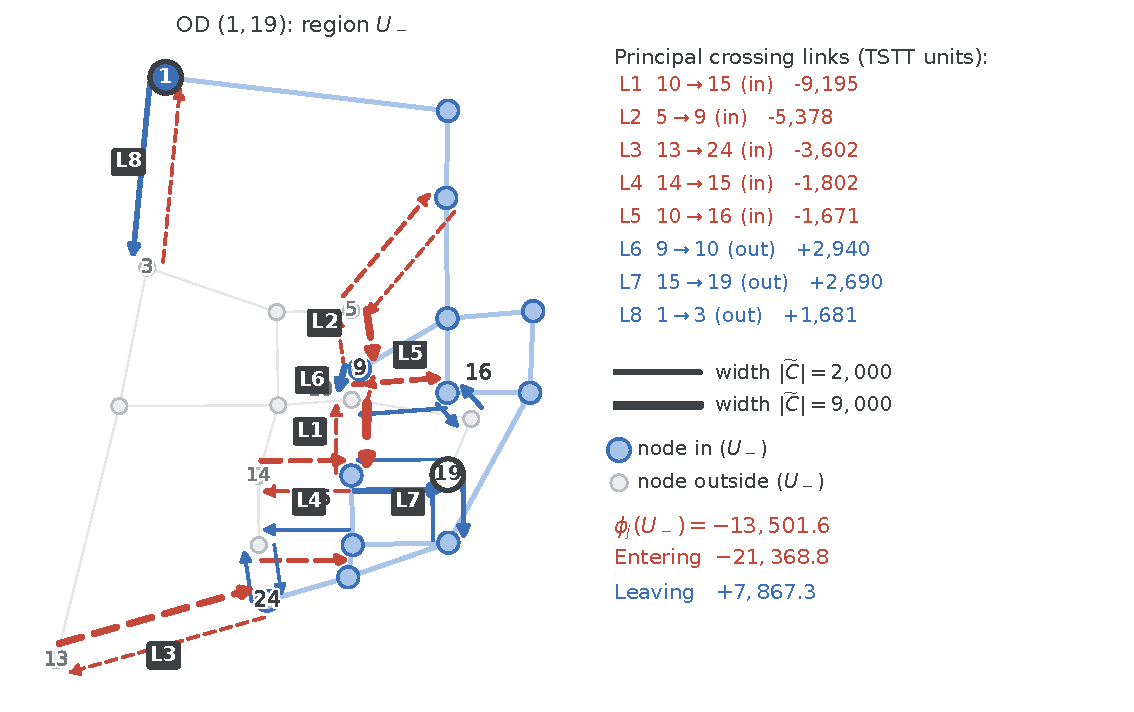
\includegraphics[width=0.82\linewidth]{../figures/fig_negmech_v102.pdf}
\caption{The connected minimizing region $U_-$ for OD $(1,19)$
(responsive-background six-query protocol). Shaded nodes form $U_-$ (origin
node $1$ ringed; destination $19$ outside). Crossing-link arrows keep
the link direction; width scales with $|c_{e,j}|$, and
colour and style encode the signed contribution to $\phi_j(U_-)$,
$a_{e,j}=\sigma_ec_{e,j}$ ($\sigma_e=+1$ leaving, $-1$
entering; solid blue positive, dashed red negative), so a positive
attribution on an entering link appears red. The side panel lists, in
TSTT units, the five largest negative and three largest positive
contributions among the $26$ crossing links
($\mathrm{L}1$--$\mathrm{L}5$ negative, $\mathrm{L}6$--$\mathrm{L}8$
positive, ``(in)''/``(out)'' marking entering and leaving links),
with the width scale and the membership legend.}
\label{fig:negmech}
\end{figure}

\FloatBarrier
\subsection{Sign preservation on the six-query baseline segment}\label{supp:screenlinelearned}
On the six-query connected families, the five flow-supervised
pretrained models (Section~\ref{supp:protocol}) show five-seed median
largest-boundary disagreements of $4.2$--$6.9\%$ of the direct
connected span for four queries, rising to $99.5\%$ for the
small-response query $(4,5)$ and beyond the span for $(7,18)$ ---
flow-only supervision does not control boundary error. Sign reliability, by contrast, is boundary specific:
all five seeds retain the three connected-family sign crossings and
positive system contributions, and at the fixed direct-model minimizing
screenline every seed keeps the negative sign for $(1,19)$ and
$(7,12)$ (seed ranges $[-3886.6,-3365.1]$ and $[-2810.4,-1916.6]$
against references $-2766.6$ and $-2967.3$, with largest family-wide
errors below the reference sign margins). These are screenline-specific
certificates of sign preservation, not of column magnitudes; the
per-query screenline table and across-seed envelopes are included in
the released result arrays.
